\let\negmedspace\undefined
\let\negthickspace\undefined
\documentclass[journal]{IEEEtran}
\usepackage[a5paper, margin=10mm, onecolumn]{geometry}
%\usepackage{lmodern} % Ensure lmodern is loaded for pdflatex
\usepackage{tfrupee} % Include tfrupee package

\setlength{\headheight}{1cm} % Set the height of the header box
\setlength{\headsep}{0mm}     % Set the distance between the header box and the top of the text

\usepackage{gvv-book}
\usepackage{gvv}
\usepackage{cite}
\usepackage{amsmath,amssymb,amsfonts,amsthm}
\usepackage{algorithmic}
\usepackage{graphicx}
\usepackage{textcomp}
\usepackage{xcolor}
\usepackage{txfonts}
\usepackage{listings}
\usepackage{enumitem}
\usepackage{mathtools}
\usepackage{gensymb}
\usepackage{comment}
\usepackage[breaklinks=true]{hyperref}
\usepackage{tkz-euclide} 
\usepackage{listings}
% \usepackage{gvv}                                        
\def\inputGnumericTable{}                                 
\usepackage[latin1]{inputenc}                                
\usepackage{color}                                            
\usepackage{array}                                            
\usepackage{longtable}                                       
\usepackage{calc}                                             
\usepackage{multirow}                                         
\usepackage{hhline}                                           
\usepackage{ifthen}                                           
\usepackage{lscape}

\newcommand{\nCr}[2]{\,^{#1}C_{#2}}

\begin{document}

\bibliographystyle{IEEEtran}
\vspace{3cm}

\title{11.16.3.8.5}
\author{EE24BTECH11012 - Bhavanisankar G S}
% \maketitle
% \newpage
% \bigskip
{\let\newpage\relax\maketitle}

\renewcommand{\thefigure}{\theenumi}
\renewcommand{\thetable}{\theenumi}
\setlength{\intextsep}{10pt} % Space between text and floats


\numberwithin{equation}{enumi}
\numberwithin{figure}{enumi}
\renewcommand{\thetable}{\theenumi}

\textbf{QUESTION} : \\
Three coins are tossed once. Find the probability of getting no head.\\
\textbf{SOLUTION} : \\

\begin{center}
\begin{tabular}{|c|c|c|}
\hline 
\textbf{Variable name} & \textbf{Description} \\
\hline 
$\vec{S}$ & Sample space \\
\hline 
$\vec{X}$ & Random variable \\
\hline
$p$, $q$ & Toss corresponding to head/tail \\
\hline
$F_{\vec{X}} (x)$ & Cumulative distribution function ( CDF ) \\
\hline
$p_{\vec{X}} (x)$ & Probability Mass function ( PMF ) \\
\hline
\end{tabular}
\end{center}

Let us assume the random variable to be the sum of three Bernoulli Random Variables.
\begin{align}
	\vec{X} &= \vec{X_{1}} + \vec{X_{2}} + \vec{X_{3}} \\
	\vec{X_{i}} &= 
	\begin{cases}
		1 & , \text{ Outcome - head } \\
		0 & , \text{ Outcome - tail }
	\end{cases} \\
	\implies p_{X_{i}} (k) &= 
	\begin{cases}
		1 - p & , k = 0 \\
		p & , k = 1
	\end{cases}
\end{align}
Considering all the outcomes as equally likely, we have
\begin{align}
	p &= \frac{1}{2} \label{eq:p}
\end{align}
For the given question, let $\vec{X}$ denote the number of heads. The sample space corresponding to the given scenario is tabulated below. \\
\begin{center}
\begin{tabular}{|c|c|c|}
\hline 
\textbf{Event} & \textbf{Sample space} \\
\hline
$p_{\vec{X}} (0)$ & \cbrak{TTT} \\
\hline
$p_{\vec{X}} (1)$ & \cbrak{TTH, THT, HTT} \\
\hline
$p_{\vec{X}} (2)$ & \cbrak{HHT, HTH, THH} \\
\hline
$p_{\vec{X}} (3)$ & \cbrak{HHH} \\
\hline
\end{tabular}
\end{center}

By the properties of Z-transform of \textbf{Probability Mass Function}, we have
\begin{align}
	M_{\vec{X}} (z) &= M_{\vec{X_{1}}} (z) M_{\vec{X_{2}}} (z) M_{\vec{X_{3}}} (z) \\
	M_{\vec{X_{1}}} &= \sum_{n \to - \infty}^{\infty} p_{\vec{X_{1}}} (n) z^{-n} = p + \brak{1-p}z^{-1} \\
	M_{\vec{X_{2}}} &= \sum_{n \to - \infty}^{\infty} p_{\vec{X_{2}}} (n) z^{-n} = p + \brak{1-p}z^{-1} \\
	M_{\vec{X_{3}}} &= \sum_{n \to - \infty}^{\infty} p_{\vec{X_{3}}} (n) z^{-n} = p + \brak{1-p}z^{-1} \\
	M_{\vec{X}} (z) &= \brak{p + \brak{1 - p}z^{-1}}^3 \\
	                &= \sum_{k \to -\infty}^{\infty} \nCr{3}{k} p^{3-k} \brak{1-p}^{k} z^{-k} \\
	p_{\vec{X}} (k) &= \nCr{3}{k} p^{3-k} \brak{1-p}^{k} \label{eq:pm}
\end{align}
Substituting \eqref{eq:p} in \eqref{eq:pm}, we have
\begin{align}
	p_{\vec{X}} (k) &= \frac{\nCr{3}{k}}{8} \label{eq:pmf}
\end{align}

The PMF is then given by - 
\begin{align}
p_{\vec{X}} (k) &= 
\begin{cases}
	\frac{\nCr{3}{k}}{8} & 0 \leq k \leq 3, k \in \mathbb{W} \\
	0 & otherwise
\end{cases} \\
\implies p_{\vec{X}} (k) &= 
\begin{cases}
	\frac{1}{8} & k = 0 \\
	\frac{3}{8} & k = 1 \\
	\frac{3}{8} & k = 2 \\
	\frac{1}{8} & k = 3 \\
	0 & \text{ otherwise }
\end{cases}
\end{align}

The corresponding \textbf{Cumulative Distribution Function} can then be written as - 
\begin{align}
	F_{\vec{X}}(k) &= Pr(\vec{X} \leq k) \\
		       &= \sum_{k=0}^{k} p_{\vec{X}} (x) 
\end{align}


\begin{align}
\implies F_{\vec{X}}(k) = Pr(\vec{X} \leq k) =
\begin{cases}
    0 & x < 0 \\
    \frac{1}{8} & 0 \leq x < 1 \\
    \frac{1}{2} & 1 \leq x < 2 \\
    \frac{7}{8} & 2 \leq x < 3 \\
    1 & x \geq 3
\end{cases}
\end{align}
\begin{align}
	F_{\vec{X}} \brak{0} &= P \brak{ \vec{X} <= 0 } \\
	                     &= \frac{1}{8}
\end{align}
\begin{figure}[h]
\centering
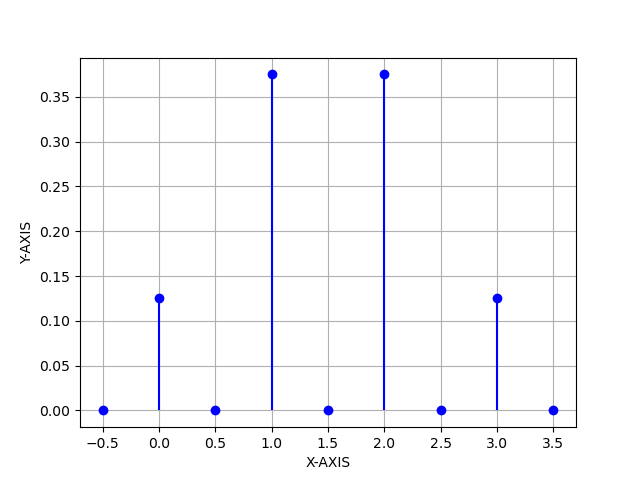
\includegraphics[width=\columnwidth]{figs/fig1.png}
\caption{Probability Mass Funtion}
\label{fig:Plot1} 
\end{figure}

\begin{figure}[h]
\centering
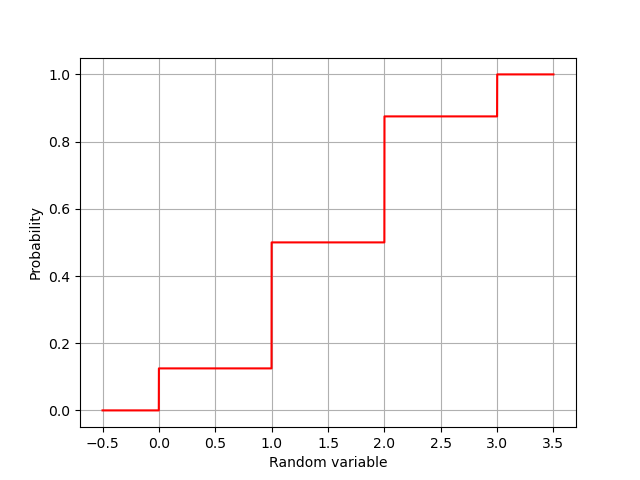
\includegraphics[width=\columnwidth]{figs/plot2.png}
\caption{Cumulative Distribution Function}
\label{fig:Plot1} 
\end{figure}

\begin{figure}[h]
\centering
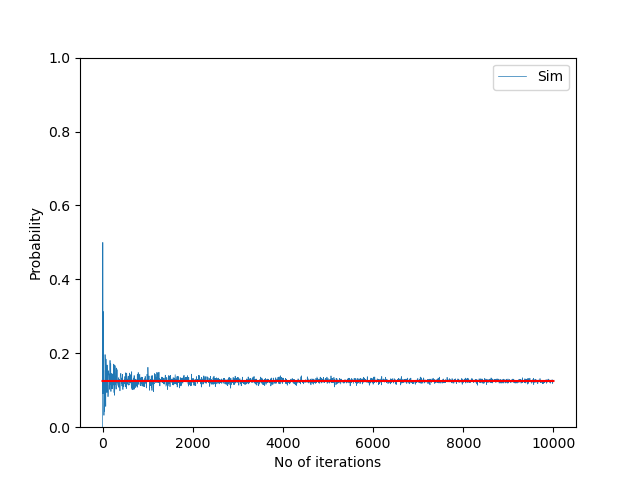
\includegraphics[width=\columnwidth]{figs/sim.png}
\caption{Simulation}
\label{fig:Plot1} 
\end{figure}
\end{document}
